% Editable vector reconstruction of the supplied figure.
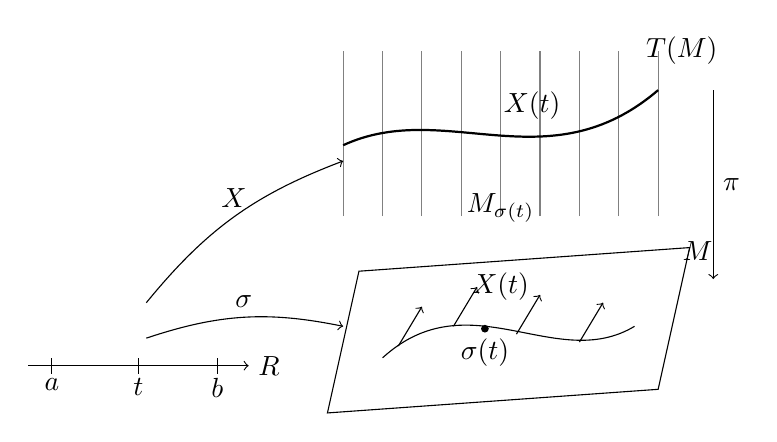
\begin{tikzpicture}
\foreach \a in {4,4.5,...,8}{\draw[gray](\a,1.9)--(\a,4);}\draw[thick](4,2.8)..controls(5.3,3.4)and(6.6,2.3)..(8,3.5);\node at(6.4,3.3){$X(t)$};\node at(8.3,4){$T(M)$};\node at(6,2){$M_{\sigma(t)}$};\draw[->](8.7,3.5)--node[right]{$\pi$}(8.7,1.1);
\draw(3.8,-.6)--(4.2,1.2)--(8.4,1.5)--(8,-.3)--cycle;\node at(8.5,1.45){$M$};\draw(4.5,.1)..controls(5.6,1.1)and(6.7,-.1)..(7.7,.5);\foreach \a/\b in {4.7/.25,5.4/.5,6.2/.4,7/.3}{\draw[->](\a,\b)--++(.3,.5);}\fill(5.8,.47)circle(1.4pt)node[below]{$\sigma(t)$};\node at(6,1){$X(t)$};
\draw[->](0,0)--(2.8,0)node[right]{$\mathbb R$};\foreach \a/\b in {.3/a,1.4/t,2.4/b}{\draw(\a,-.1)--(\a,.1)node[below=4pt]{$\b$};}\draw[->](1.5,.35)to[bend left=15]node[above]{$\sigma$}(4,.5);\draw[->](1.5,.8)to[bend left=15]node[above]{$X$}(4,2.6);
\end{tikzpicture}
